\chapter{Study design and experiments}
\label{chp:inf-max}

In this chapter, we present the design of the study and the experiments performed to further the research in the domain of influence mining. Recall from chapter \ref{chp:related-work} where we showed that the problem of identifying most influential nodes in a graph is a global optimization problem. The objective is to find a set $S$ such that there is no other set which maximizes the influence more than $S$. It also proved that this is a difficult problem to solve optimally in real world scenarios. There have been numerous attempts to solve this problem, which has been covered in chapter \ref{chp:related-work} with mixed results but a generalized solution -- one which works for all use cases of influence mining problems -- is still awaited. We attempt to perform various experiments to discover and propose a realistic solution to the influence mining problem.

	\section{Study design}
	Figure \ref{fig:study-design} sums up the study from inception of the problem to proposed solution. Each block in the diagram is expanded into a section of this chapter, starting from data collection to the solution framework.

	\begin{figure}[H]
		\centering
		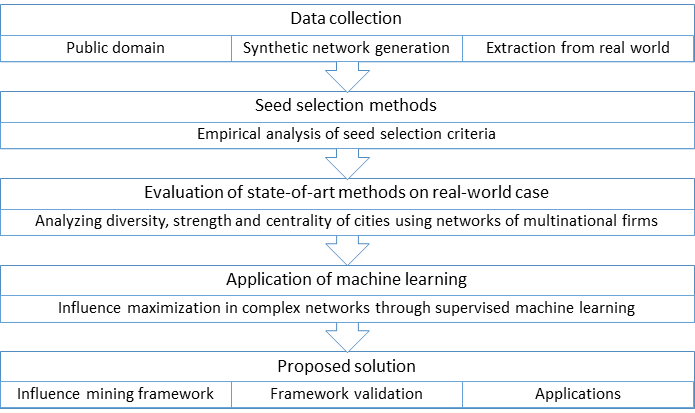
\includegraphics[width=1\textwidth]{study-design}
		\caption[Experiment design]{Study design representing flow of the study from inception to conclusion.}
		\label{fig:study-design}
	\end{figure}
	
		\subsection{Data collection}
		Experiments discussed in this chapter use various network data sets which are obtained from different domains. There are three main sources of the data:
		
		\begin{enumerate}
			\item Public domain: these data sets are collected from public sources. The rationale behind using these data sets is that they appear frequently in past as well as state-of-art researches. In addition, these are in clean, pre-processed form with structural properties already known.
			
			\item Synthetic: such networks are generated via network generator tools. As explained in \ref{sec:domain-synthetic-nets}, they imitate behaviour of real networks but do not contain real-world bias as well as come in handy for bootstrapping purpose when there is scarcity of real-world data.
						
			\item Extracted: some of the networks used have been collected by the author or associates directly from real-world implementations. The primary purpose of these networks is to test methodologies on actual use cases which contain real-world noise and biases.			
		\end{enumerate}
	
		\subsection{Seed selection methods}
		We performed a number of experiments with real world and synthetic networks. The objective of these experiments was to test several seed selection methods used in the literature and analyze whether influence depends only on the structure of a network, or do seed selection methods play a role in spreading influence in different types of networks.
		
		\subsection{Evaluation of state-of-art methods on real-world case}
		Learning from previous experiment, it was established that the seed selection criteria can vary in performance if the structure of network is different. On the other hand, a variety of methods were proposed by the research community, each claiming to outperform existing methods. This experiment was conducted to test CI, a state-of-art seed selection algorithm against known popular methods. The study compares findings with ground truth on multiple dimensions including diversity, strength and centrality of nodes.

		\subsection{Application of machine learning}
		Failing to identify a single heuristic to extract influential nodes in all kinds of networks, we modeled the problem as a supervised machine learning problem, which is a data mining technique. The object was to combine the strengths of multiple seed selection methods and classify influential nodes on various networks to construct a general purpose influence mining model. We started from generating a dataset, consisting of macro and micro level details as features and target labels (influential/non-influential) identified through optimal and greedy algorithms. In the second phase, we trained multiple models, and selected the most accurate model to further test on real-world networks. The study concludes that machine learning is a viable solution to the influence maximization problem for a broad variety of networks with varying structural properties.

		\subsection{Proposed solution}
		Combining the feedback from all experiments performed, it was evident that not only there is an absence of one algorithm which can satisfactorily solve the influence mining problem, but also that existing research focuses only on a single convergence criteria when choosing an influence mining algorithm. Moreover, the algorithms themselves are tested by quantifying the diffusion alone. We argue that both of these fixed settings do not fully address the real-world problems and propose a framework in response which addresses these key observations.


	%%%%%%%%%%%%%%%%%%%%%%
	%%% Experiment - 1 %%%
	%%%%%%%%%%%%%%%%%%%%%%
	\section{Empirical analysis of seed selection criterion}
	\label{sec:inf-max-seed-selection-analysis}
	The foundations of the contribution in this experiment were laid by Hashmi et. al. \cite{hashmi2012} who targeted five semantically different social networks as described in Table \ref{tab:inf-max-social-networks}. These networks were randomly sampled ten times and their statistics were averaged; then these networks were compared using three levels: elemental, group-level and network-level\footnote{These terms are synonymous to the levels discussed in \ref{chp:domain}, i.e. Elementary is Micro-level, Group is Meso-level; Network is Macro-level}. Their results found the networks under observation to be structurally similar with a few exceptions.
	
	\begin{table}[h]
		\centering
		\begin{tabular}{|l|l|l|l|l|l|l|l|}
			\hline
			& \textbf{Edges} & \textbf{Density} & \textbf{HD} & \textbf{Diameter} & \textbf{CC} & \textbf{APL} & \textbf{$\alpha$} \\ \hline
			\textbf{Twitter}   & 3099  & 6.18  & 237 & 11 & 0.19 & 2.6  & 1.57 \\ \hline
			\textbf{Epinions}  & 13739 & 27.47 & 278 & 7  & 0.43 & 1.93 & 1.2  \\ \hline
			\textbf{Wikipedia} & 11672 & 23.34 & 281 & 12 & 0.35 & 2.1  & 1.21 \\ \hline
			\textbf{Email}     & 2396  & 4.79  & 499 & 7  & 0.54 & 1.98 & 1.87 \\ \hline
			\textbf{Co-Author} & 2404  & 4.8   & 102 & 10 & 0.6  & 2.87 & 1.66 \\ \hline
		\end{tabular}
		\caption[Networks statistics of social network data sets]{Networks statistics of social network data sets used. The networks are sampled with size 500 each. HD is highest degree, CC is graph clustering coefficient, APL is average path length and $\alpha$ is the power-law coefficient}
		\label{tab:inf-max-social-networks}
	\end{table}
	
	While the overall results stayed as expected, i.e. the networks exhibited similar structural properties despite being contextually different. However, the authors observed a few exceptions, as shown in Figure \ref{fig:structural-similarity}. The variation in Clustering coefficient and Strength of triads show some structural dissimilarities. For example, in case of email network, the CC is spread across the network rather than lying in core of the network as others. The linear decay in degree distribution for Epinions and Wikipedia networks indicated non-scale free behaviour. And final dissimilarity flagged was that the Closeness centrality significantly varied for email network, suggesting that the very high value of HD caused the drop in closeness for other nodes.
	
	\begin{figure}[H]
		\centering
		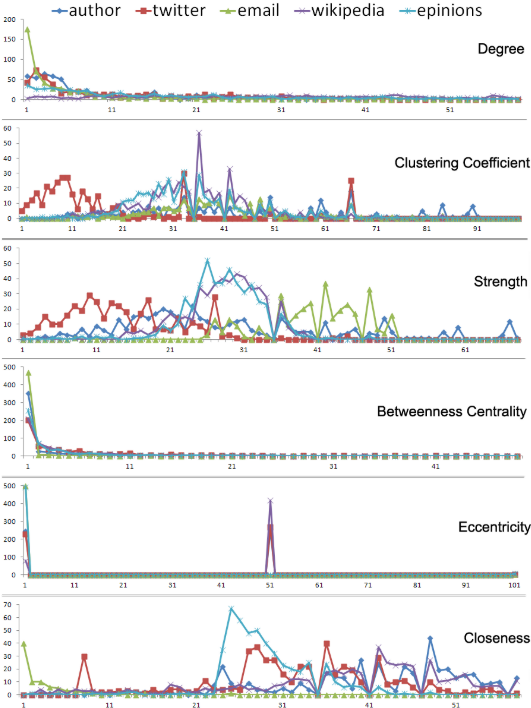
\includegraphics[width=0.7\textwidth]{structural-similarity}
		\caption[Frequency distribution of seed selection metrics of five networks]{Frequency distribution of network metrics. Horizontal axes shows bins of metric values and vertical axes represent frequency of node occurrences \cite{hashmi2012}.}
		\label{fig:structural-similarity}
	\end{figure}
	
	Following the lead from this study, we conduct an empirical experiment \cite{hussain2013a} to closely observe the impact of various seed selection methods on both IC and LT diffusion models on both real and synthetic networks. For diversification, four classes of networks were selected: scale free, small-world, scale free and small-world and random.
	
	%Starting with an undirected graph $G=(V,E)$, each edge $E=(u, v)$ represents that nodes $u$ and $v$ have a direct edge with each other. For IC model, we use chance probability (0.5) to exert influence from active nodes on their inactive neighbours. An inactive neighbour is influenced only once with this probability; consequently, it will either activate and further spread action $a$ or stay inactive. Either way, a node will not be tried for activation twice. In the LT model, each inactive node looks for active nodes in its neighbourhood and if the incoming influence from neighbourhood is above certain activation threshold, the inactive node will also become active.
	
	In given Algorithm \ref{alg:seed-selection}, $G=(V,E)$ is the prerequisite network, $k$ is some budget, $M$ is any function to calculate centrality of nodes ($M_v$ represents centrality of a single node; $M_{V}$ means centrality of all nodes in $V$) and $\sigma$ is a function to calculate the spread or influence of selected seed set. Note that instead of learning influence probabilities, we used chance probability (0.5).
	
	\begin{algorithm}[h]
		\caption{Diffusion algorithm using various seed selection methods}
		\label{alg:seed-selection}
		\SetAlgoLined
		\KwInput{$G:(V,E);k\leq|V|;M;\sigma$ (given a connected graph $G$ of $V$ vertices and $E$, budget $k$, a function $M$ to compute node centrality; influence quantifier $\sigma$)}
		\KwOutput{$\sigma$ (the number of nodes influenced successfully)}
		$S \leftarrow \emptyset$; $\sigma \leftarrow 0$
		\newline
		\While{$|S|<k$}{
			$S \leftarrow S \cup (v|M_{v}=max(\{M_{s}\})$ (pick the node $v$ with maximum centrality value in remaining nodes)
		}
		$W \gets V-S$
		\newline
		\While{$W \neq \emptyset$}{
			$A \leftarrow \emptyset$
			\newline
			\For{$v \in W$}{
				$N \leftarrow u|u \in S; (u,v)=1$; $\theta \leftarrow rand(0,|N|)$
				$sum \leftarrow \Sigma_{i=1 to |u|} j=rand(0,1)$ (toss a coin for each neighbour and sum up the number of successes)
				\newline
				\If{$sum \geq \theta$}{
					$A \leftarrow A \cup {v}$
				}
				$W \gets W-{v}$
			}
			$S \leftarrow S \cup A$; $\sigma \leftarrow \sigma + |A|$
		}
		\Return{$S,\sigma$}
	\end{algorithm}

	First phase of the algorithm executes a loop. In each iteration, a node with highest centrality score is picked and added to seed set $S$. The next phase runs iteratively until no nodes are left which have not been attempted for activation. The nodes activated successfully by $S$ are removed from graph iteratively; each node $u$ attempts to activate inactive nodes in $v\in V$ by chosing a random threshold. If the total sum of active nodes in $S$ who have successfully attempted to activate $v$ exceeds this threshold $\theta$ then $v$ is activated and added to the set $S$ for next iteration. When the loop ends, all $v$ nodes which have been attempted are removed as they will never be activated again. The influence is then recalculated based on newly activated nodes in $S$. At the end, total influence $\sigma(S)$.
	
		\subsection{Experiment settings} 
		The experiment performed for empirical analysis of seed selection methods uses both real and synthetic networks. The networks generated were small world (SW) using the model from \cite{watts1998}, scale free (SF) using the model from \cite{barabasi1999}, small world-scale free network (HK) using the model of \cite{holme2002} and random network (RD) using the model network of \cite{erdos1960} to represent different types of networks. Small world model can be generated for the desired number of nodes and edges by starting with a regular graph in which each node has a degree $n$. In scale free model nodes are attached preferentially therefore for every new node we can tune the number of edges to make a scale free network. Small world-scale free model can also be tuned by the number of nodes to which each new node connects to, which will give us the desired edge-node ratio. We have generated a random network with $n$ nodes and $m$ edges whose degree distribution $p_k$ follows the Poisson distribution $p_k = e^{-\lambda} \frac{\lambda^k}{k!}$ . In our generated networks , all had $\lambda > 1$ which indicates that most nodes have the degree close to the mean degree of the network.
		
		The real networks include Political Blog, Twitter, Epinions and Author networks which are briefly described below:
		
		\begin{enumerate}
			\item Political Blog: hyperlinks network between weblogs on US politics, which was recorded in 2005 by Adamic and Glance \cite{adamic2005}. Each node represents a blog post while an edges are links between blogs, which were automatically detecting by crawling the links on front page of blogs.
			
			\item Twitter: famous micro-blogging social network. The data set used is originally extracted by \cite{hashmi2012}. A node is a registered user account, while an edge between two nodes means any one or both users have followed the other.
			
			\item Epinions\footnote{\url{http://snap.stanford.edu/data}}: a who-trust-whom online network at Epinions.com, a customer analysis website. To trust each other, site members can either agree or disagree. Trust is formed by the interaction of all the reliable contacts which is on the basis of review ratings.
			
			\item Author\footnote{\url{http://vlado.fmf.uni-lj.si/pub/networks/data/}}: a co-authorship network, generated from the BibTeX bibliography developed from the Computational Geometry Database. Each author is a node and two authors form an edge if they have contributed to same work together, e.g. an article, book etc.
		\end{enumerate}
		
		The real data sets were reduced to the largest connected components. Then, the synthetic networks were generated equivalent to the real networks in structure, i.e. five simulated networks for each class equivalent to the four real social networks, summing up to a total of 80 networks. The rationale behind selecting multiple data sets for experimentation is to ensure accuracy, since the information diffusion in each model is based on random choices (see Table \ref{tab:inf-max-social-networks-2}). An important similarity among all these networks is the low average path length and high clustering coefficients of these networks giving them small world properties except random networks. Scale free networks have low clustering coefficient and the degree distribution of small world and random networks follows a Poisson distribution with $\lambda >1$. As an example, Table \ref{tab:inf-max-empirical-analysis-apl} explains how the APL of these networks compare.
		
		\begin{table}[h]
			\centering
			\begin{tabular}{|l|l|l|l|}
				\hline
				& \textbf{Nodes} & \textbf{Edges} & \textbf{Density} \\ \hline
				\textbf{Blog}     & 1222           & 16714          & 13.6             \\ \hline
				\textbf{Twitter}  & 2492           & 17658          & 7                \\ \hline
				\textbf{Epinions} & 2000           & 48720          & 24.3             \\ \hline
				\textbf{Author}   & 3621           & 9461           & 2.6              \\ \hline
			\end{tabular}
			\caption{Size, number of edges and density of the four real networks used.}
			\label{tab:inf-max-social-networks-2}
		\end{table}
		
		\begin{table}[h]
			\centering
			\begin{tabular}{|l|l|l|l|l|l|}
				\hline
				\textbf{Data set} & \textbf{Real} & \textbf{RD} & \textbf{SW} & \textbf{SF} & \textbf{HK} \\ \hline
				\textbf{Blog}     & 2.7           & 2.5         & 3.2         & 2.4         & 2.2         \\ \hline
				\textbf{Twitter}  & 3.4           & 3.2         & 4.2         & 2.9         & 2.8         \\ \hline
				\textbf{Epinions} & 2.2           & 2.2         & 3           & 2.2         & 2           \\ \hline
				\textbf{Author}   & 5.31          & 5.07        & 6.41        & 3.4         & 4           \\ \hline
			\end{tabular}
			\caption{RD, SW, SF, HK mean that synthetic network was extracted using a synthetic network generator using: Random model, Small-world model, Scale Free model, and Holme and Kim Model (small world-scale free networks) respectively. The value represents average APL for each class in all real and generated networks.}
			\label{tab:inf-max-empirical-analysis-apl}
		\end{table}
		
		\subsection{Results}
		Figure \ref{fig:empirical-analysis-influence} describes the influence spread as well as the iterations it took for each method to reach all nodes. There are some key findings from this experiment, as evident from results:
		
		\begin{itemize}
			\item The first observation from the results of influence spread is that the behavior of small world networks and random networks is the same for all the different seed selection strategies with a lone exception of closeness centrality on Twitter. The reasons here is an important similarity in small world networks and random networks; their APL is low, but since both of these two classes of complex networks are missing very high-degree nodes, the algorithms behaves similarly for all the different seed selection methods.
			
			\item Small world networks have high clustering coefficient due to abundance of triads. On the other hand, random networks have scarcity of triads. It is therefore expected for small-world networks to exhibit high influence spread, but to our surprise, no significant impact of clustering coefficient was evident during our experiments; rather, high-degree nodes contributed more in the influence spread.
			
			\item In real networks, scale free networks (SF) and small world-scale free networks (HK), the betweenness centrality leads the other metrics in spreading maximum influence followed closely by degree centrality.
			
			\item Closeness performs well for the Twitter network whereas for the other three data sets, the closeness and random selection have only minor differences.
			
			\item Eigen-vector performs well for small world-scale free and scale free networks, even better than betweenness centrality for the Epinions network. Interestingly, the Eigen-vector centrality is quite variable in performance on real networks. It performs poorly for Twitter network, worse than closeness. It performs very close to betweenness and degree centrality for Epinions and has a notable difference for Blog and Author networks.
			
			\item The similarity between real networks and HK are notably high. This reaffirms that most real world networks are both small world and scale free in nature. An exception to this narrative is Author data set, but it can be argued that this is due to the marginal difference in high degree. Original network has high degree 102, while its SF and HK counterparts have 201 and 183 respectively.
			
			\item In terms of iterations, betweenness centrality performs well along with degree and eigen-vector centrality except for the case of small world and random networks generated equivalent to the Author network. An exception again, is Author network which required more iterations. However, this time it is due to the density of the network as well as relatively low value of high-degree node. Epinions networks also proves the above conjecture, as the highest degree node in the real Epinions network is with degree 1192, which is more than 50\% of the nodes are connected to a single node.
			
			\item The edge density and the number of iterations show signs of negative correlation; the most dense network (24.3) of Epinions took an average of 2.4 iterations; Political Blog network with density of 13.6 averaged 3.0 iterations; Twitter with a density of 7 finished iterating with an average 3.6; the Author network of density only 2.6 took most average iterations of 4.8. Concisely, the denser a network is, the less iterations it takes for influence process to complete.
			% The above point was indicated by Dr. Guy Melancon in his review feedback
			
			\item Lastly and as expected, the APL exhibited uniform behaviour in almost all the experiments. The number of iterations on all of the Epinions and Blog data sets, having low APL remained between 2 and 5. Twitter data set took 6 iterations for RD in random influence method and 5 iterations for the rest of the methods. However, on Author data set with highest APL, the number of iterations begin from 4 and hike to 8. This is because it requires less number of steps to traverse from one node to another in the network.
		\end{itemize}
		
		\begin{figure}[H]
			\centering
			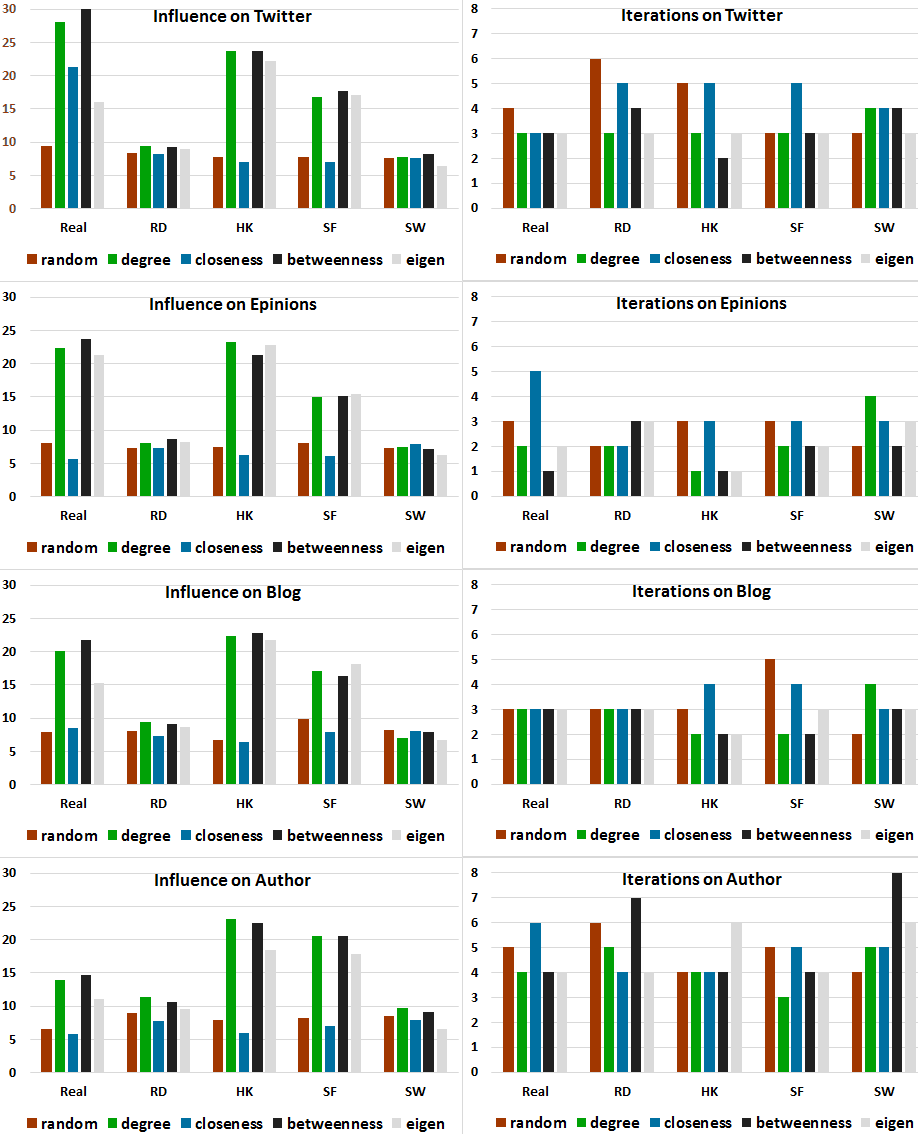
\includegraphics[width=0.8\textwidth]{empirical-analysis-influence}
			\caption[Influence spread and number of iterations on networks]{Figure showing bar graphs for the data sets and their simulated networks. Bars on the left side represent the average percentage of total nodes influenced during diffusion process with budget $k=5\%$. Bars on the rights side represent the average number of iterations that the algorithm took to try to spread the influence to whole network. The results are aggregate of all 80 networks generated.}
			\label{fig:empirical-analysis-influence}
		\end{figure}
		
	The key finding from the above experiment is that the seed selection criteria plays less important role than the structure of the network itself in the influence maximization process. Thus solidifying the conjecture that a certain seed selection method can vary in performance on different types of networks.
	
	In the next section, we scrutinize influence mining phenomenon from an application perspective on a real-world case. The aim is not only to see if a state-of-art method outperforms classic heuristics, but also to analyze whether the conclusions drawn from influence maximization method actually match with the ground truth.

%	\newpage

	%%%%%%%%%%%%%%%%%%%%%%
	%%% Experiment - 2 %%%
	%%%%%%%%%%%%%%%%%%%%%%
	\section{Analyzing Diversity, Strength and Centrality of Cities using Networks of Multinational Firms}
	\label{sec:resilience-city-networks}
	In this experiment, we put the resilience methods to test in a real world scenario \cite{hussain2019}. The main objective is to test whether resilience methods are able to successfully identify critical cities in global economic networks. Once the methods were able to identify the critical cities, we studied the economic networks over two time periods 2010 and 2013 to analyze the change in the importance of cities over the two time periods. Secondarily, we observe different influence mining methods and see which of them is more appropriate for further analysis. We analyze diversity, strength and centrality of the cities considering these as key indicators in observing how cities have changed their roles in the global economic networks over time.
	
	In particular, we are looking for the aftermath of great recession that occurred in 2008. Unsurprisingly, this is a very well established field of research and there have been numerous studies focusing specifically on city importance under the lens of economic ties \cite{blumenfeld2009,storper1997,scott2003}. The application of network analysis is also not novel in this area, \cite{barabasi1999,ducruet2014,liu2014} have observed the cities as complex networks before, and have confirmed that the economic ties between cities cause a ripple effect between strongly linked cities when one city is affected both positively and negatively. In particular, \cite{derudder2003,liu2014} explored the hierarchical organization of cities; \cite{taylor2002,taylor2013,alderson2004} focus on topological view of these cities; \cite{sassen2007,sassen2011} study city networks from the perspective of spatial concentrations forming economic hubs; closely tied to the financial hubs, \cite{ducruet2011,beaverstock2002} explore the densely connected components, often referred to as communities in SNA, especially \cite{liu2014} applied hierarchical community detection to find hierarchical and temporal patterns.
	
	The application of resilience problem on city networks although is not new in this arena, it is rare to some degree. Barthélemy \cite{barthelemy2011} and Okelly \cite{okelly2014} have previously explored the resilient cities in search of identifying most dominant economies. In this regard the rise of China as a global economic power, as well as the Gulf region is widely studied and accepted \cite{alderson2010,mahutga2010,derudder2010}. Our findings re-assert this rise between 2010-2013; however the main objective is to identify other cities and global regions which exhibit similar significance but are either non-trivial to find, or are overlooked.
	
		\subsection{Data set}
		The underlying experiment uses a data set consisting of two networks from year 2010 and 2013 of economic ties of multinational firms and their subsidiaries. Each node represents a city\footnote{The term city is used loosely here, they actually represent a large urban area delineated with the a standard criteria (see \cite{rozenblat2017}). For example, Paris represents all the smaller towns and cities located around it.} where an edge is an ownership connection between two organizations located in the cities, i.e. if two cities have an economic and financial link and belong to the same group of companies, an edge is formed. The world's leading 3000 multinational groups of companies with 800,000 direct and indirect subsidiaries are used to build the network, forming 1 million edges between them. The top group of companies were selected based on their annual turnover and made available by Bureau van Dijk\footnote{Bureau van Dijk Electronic Publishing (\url{http://www.bvdep.com/)}}.
		The data has been extensively processed to clean incorrect fields and complete missing values at the Universit\'{e} de Lausanne - ERC GeoDiversity research group\footnote{ORBIS 2010, 2013: BvD - Universit\'{e} de Lausanne, ERC - Geodiversity, Switzerland)}. These networks are similar in construction but larger in size to other datasets \cite{kraetke2014,wall2011,alderson2004} extensively used to represent economic networks of cities. Figure \ref{fig:city-network-construction} depicts the construction of these networks. Table \ref{tab:resilience-city-network-stats} shows a quantitative summary of different measures for the two networks constructed, one for the year 2010, and the other for 2013.
		
		\begin{figure}[H]
			\centering
			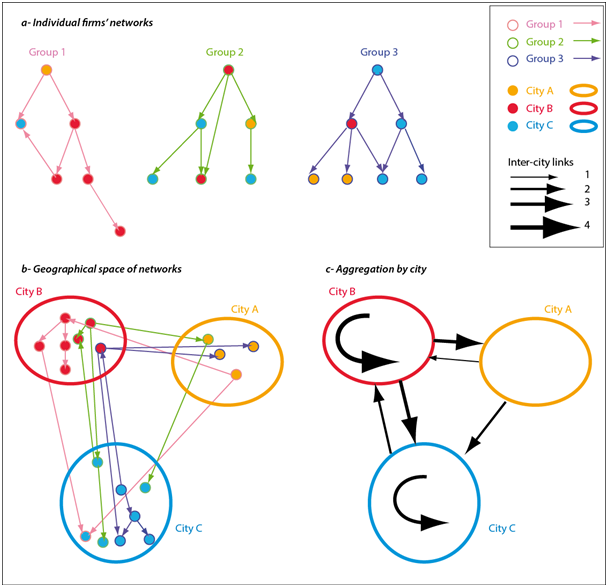
\includegraphics[width=0.8\textwidth]{city-network-construction}
			\caption[Hierarchy of economic network of multinational firms]{Construction of Economic Networks of Cities: (a) Hierarchy of Multinational Firms and the links to their Subsidiaries (b) Firms are Geographically Distributed and (c) Links are aggregated to connect cities forming Economic Networks. \cite{rozenblat2017}}
			\label{fig:city-network-construction}
		\end{figure}
	
		The networks have high similarity in highest degree and transitivity measures. While transitivity tells how many triads of cities are there, highest node degree explains the maximum number of unique connections a city has with others.
		
		A key observation from 2010 to 2013 is that the number of new nodes and connections have grown, which is a hint on how the multinational firms are opting their strategy of expansion. This could be caused due to two main reasons: either the firms have opened new franchises or acquired new partners to increase their footprint, or they have risen to the top 3000 multinational companies in 2013, and are therefore reflected in new network
		
		\begin{table}[h]
			\centering
			\begin{tabular}{|l|l|l|}
				\hline
				\textbf{Metric}                     & \textbf{2010} & \textbf{2013} \\ \hline
				Cities (Represented by Nodes)       & 1206          & 1253          \\ \hline
				City-City Linkage (Unweighed Edges) & 28639         & 31704         \\ \hline
				Node-Edge Ratio                     & 23.7          & 25.3          \\ \hline
				Highest Degree                      & 762           & 777           \\ \hline
				Average Path Length                 & 2.29          & 2.27          \\ \hline
				Transitivity                        & 0.331         & 0.339         \\ \hline
			\end{tabular}
			\caption[Quantitative comparison of the both instances of city networks]{Network Statistics: Quantitatively comparing the two networks. Different network metrics show the structural similarity of the two networks.}
			\label{tab:resilience-city-network-stats}
		\end{table}
	
		\subsection{Experiment settings}
			
			\subsubsection{Diversity, Strength and Centrality}
			To define the importance of a city, three notions are used, namely \textit{Diversity}, \textit{Strength} and \textit{Centrality}:
			
			\begin{enumerate}
				\item Diversity: we describe Diversity as a measure of importance of a city based on the number of connections it has to other unique cities\footnote{In SNA, Diversity can be calculated using Unweighted Degree Centrality}. For example, in figure \ref{fig:city-network-construction} $A$ has three connections with $B$, and single connection with $C$, in terms of diversity. We would therefore say that the diversity of $A$ is 2.
				
				\item Strength: Strength\footnote{Weighted Degree is used to calculate Strength} reflects the total number of connections a city has in the network. Continuing with our example, city $A$ would have a strength of 4 as it has a total of 4 connections, 3 with city $B$ and 1 with city $C$. The higher the number of ties it has with other cities, the stronger it is in the network.
				
				\item Centrality: Centrality is arguably the most widely used metric in network analysis. We used two approaches to compute centrality, first from Global Production and Value Networks \cite{henderson2002,gereffi2005}, which are common in spatial economics, and the other from network connectivity \cite{brandes2005} which is more generic.
			\end{enumerate}
		
			The cities which connect global network are considered pivotal. This in turn can be represented by cities which hold the network together as a single connected network. We estimate this by using the network dismantling method discussed in \ref{sec:domain-resilience}. This connectivity is critical in avoiding economic silos which hinder global trade and economic development thus putting cities with this characteristic in a central position.
		
			Learning from the classical and state-of-art literature, it is clear that no single metric has been proven to be most effective in finding central nodes in different network topology. Since centrality varies based on the topology and structure of a network \cite{hashmi2012,hussain2013a,malighetti2019}, we applied several metrics extensively used in the literature to find the optimal metric for each of the two city networks used in this study.
		
			We used Degree Centrality, Betweenness Centrality, Eigenvector Centrality, Pagerank, K-shell decomposition and Collective Influence to represent a wide array of state-of-art methods. Moreover, along with their baseline use, we added Adaptive sampling technique (see \ref{sec:related-seed-selection}) to each of these methods because of its general effectiveness. Algorithm \ref{alg:adaptive-sampling} represents the adaptive variation to calculate central nodes representing cities for any given metric.
			
			\begin{algorithm}
				\caption{Adaptive variation \cite{lipton1989} to calculate central cities using certain metric}
				\label{alg:adaptive-sampling}
				\KwInput{$G:(V,E);M$ (given a connected graph $G$ of $V$ vertices and $E$, budget $k$, and a method $M$ to calculate centrality)}
				\KwOutput{$S$ (the set of central cities)}
				$S\gets \emptyset$
				\newline
				$W\gets V$
				\While{$|W|>0$}{
					$v_{max}\gets v|v\in{W}, M_v=max(\{M_W\})$; $S\gets S \cup v_{max}$
					\newline
					$G\gets largest\_connected\_component(G(W-v_{max}))$
					\newline
					$W\gets vertices_{of}(G)$
				}
				\Return{$S$}
			\end{algorithm}
		
			Figure \ref{fig:city-network-metrics} compares the performance of the various metrics on the two networks along with their adaptive variations. Figure \ref{fig:city-network-dismantling} depicts the progression of network dismantling process for top four metrics. A metric is deemed to perform better than the other if it requires less number of iterations, which implies that fewer of cities (nodes) where removed from the network to completely disintegrate it. As clearly visible, Adaptive Betweenness outperformed other methods in central node identification in both networks. This is partly consistent with the approach proposed by \cite{henderson2002} where the authors provide an alternate network construction and use the classical Betweenness Centrality (as opposed to the adaptive version described here) to identify the importance of cities in the world city network.
			
			\begin{figure}[H]
				\begin{subfigure}{0.5\textwidth}
					\centering
					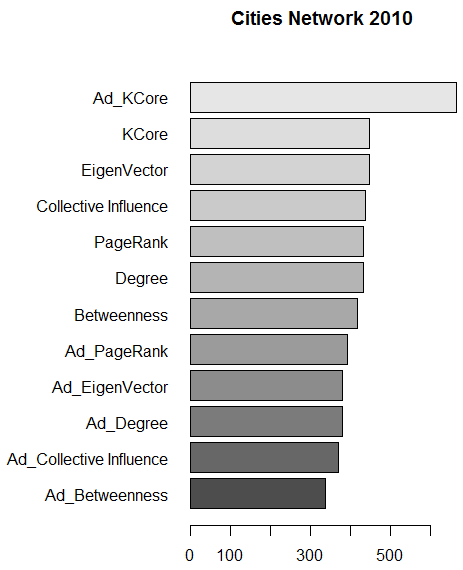
\includegraphics[width=1\linewidth]{city-network-metrics-2010}
					\label{fig:city-network-metrics-2010}
				\end{subfigure}%
				\begin{subfigure}{0.5\textwidth}
					\centering
					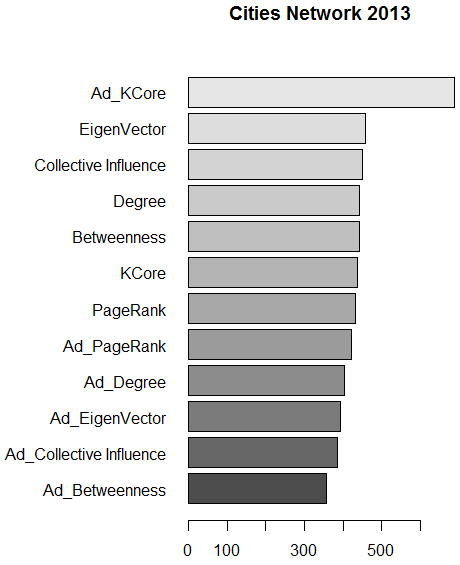
\includegraphics[width=1\linewidth]{city-network-metrics-2013}
					\label{fig:city-network-metrics-2013}
				\end{subfigure}
				\caption[Comparison of network metrics to identify for city networks]{Comparison of network metrics to identify the most effective method for networks of 2010 and 2013. Metrics are sorted by the lowest performing to the best performing from top to bottom. X-axis represents the number of node removals required to completely disintegrate the entire network whereas Y-axis represents the size of the biggest connected component in the network. Prefix \textbf{Ad} with different metrics represents the adaptive sampling variant.}
				\label{fig:city-network-metrics}
			\end{figure}
			
			\begin{figure}[H]
				\begin{subfigure}{0.5\textwidth}
					\centering
					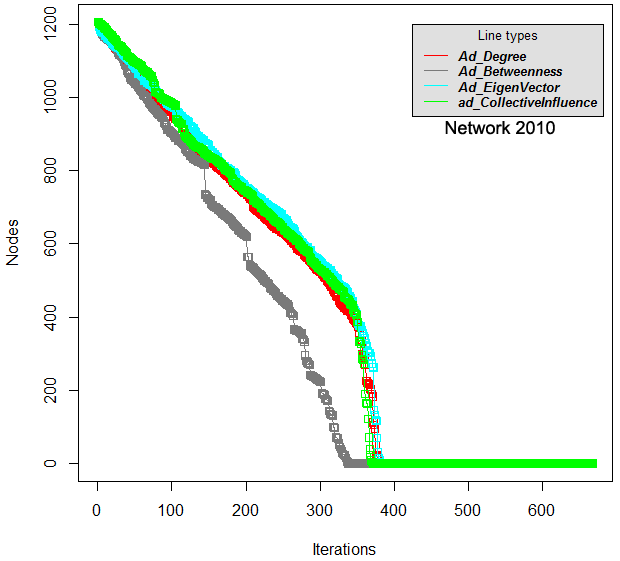
\includegraphics[width=1\linewidth]{city-network-dismantling-2010}
					\label{fig:city-network-dismantling-2010}
				\end{subfigure}%
				\begin{subfigure}{0.5\textwidth}
					\centering
					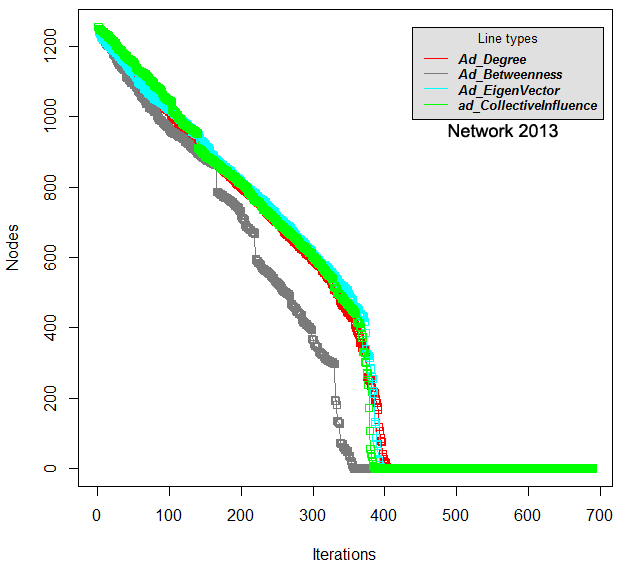
\includegraphics[width=1\linewidth]{city-network-dismantling-2013}
					\label{fig:city-network-dismantling-2013}
				\end{subfigure}
				\caption[Comparing the four best metrics to determine network connectivity]{Comparing the four best metrics to determine network connectivity. On x-axis is the number of iterations which a method took to dismantle the network; on y-axis is the number of remaining nodes in the largest component of the network. As seen, the Adaptive Betweenness heuristic outperformed the other methods by dismantline the network faster in both networks.}
				\label{fig:city-network-dismantling}
			\end{figure}
		
			\subsubsection{Cumulative city rankings}
			The importance of cities cannot be determined by a single metric because all Diversity, Strength and Centrality measures highlight the vitality of a city. These three metrics -- originally inspired by social network analysis -- have formed the basis of many research studies to quantify the role of cities in the world economy \cite{alderson2004,derudder2010,rozenblat2017}. As there's no order in which these metrics can be used, we propose a cumulative rank ($CR$) which combines all three to ensure an unbiased representation of various dimensions studied in this section. The cumulative rank is weighed equally by taking harmonic mean: $CR_i=\frac{n}{\sum_{i=1}^{n} \dfrac{1}{x}}$. The harmonic mean of a city $i$ given by $CR_i$ is calculated by using the rank of city $x$ for each of the three metrics ($n=3$) such that $x_1$, $x_2$ and $x_3$ represent the rankings in the three metrics. The cumulative rank ensures that the importance of a city is measured along all three dimensions, thus building a fair basis for interpretation of results.
	
		\subsection{Results}
		First and most important finding is the fact that on this real world network, neither a traditional, nor a state-of-art method proved to be the best in finding the most central nodes. The experiments on networks reveal that Adaptive sampling method of Betwenneess Centrality outperforms the other metrics in identifying the most central nodes.
	
			\subsubsection{Diversity}
			Figure \ref{fig:city-network-diversity} shows the diversity of cities in 2010 and 2013. The cities which are very close to the trend line have maintained their status from the year 2010 to 2013. Almost all the top cities like \textbf{Paris}, \textbf{New York} and \textbf{Tokyo} have shown this tendency which reflects that in terms of diversity, not much changed during the studied period. The cities which are far below the trend line have decreased in terms of diversity. Major cities affected in this way are \textbf{Frankfurt}, \textbf{Copenhagen}, \textbf{Stockholm} and \textbf{Rome}. Cities which are above the trend line such as \textbf{Milan}, \textbf{Geneva} and \textbf{Baltimore} have increased their diversity over the period and now have more connections to different cities. Cities of \textbf{Scandinavia} (like Copenhagen, Stockholm, or Goteborg) or cities of \textbf{South} (like Roma, Barcelona) mostly decreased while cities situated at the center like \textbf{Zurich}, \textbf{Geneva}, \textbf{Milano}, or \textbf{Mannheim} increased. Because of the crisis, networks have a tendency to concentrate in some geographic central cities, despite the observed exception of Frankfurt hosting the European central bank which had the opposite effect of weakening the city.
			
			Also interesting mention here are the cities of \textbf{Dubai} and \textbf{Abu Dhabi} which have also increased considerably representing growth in the Gulf region.
			
			\begin{figure}[H]
				\centering
				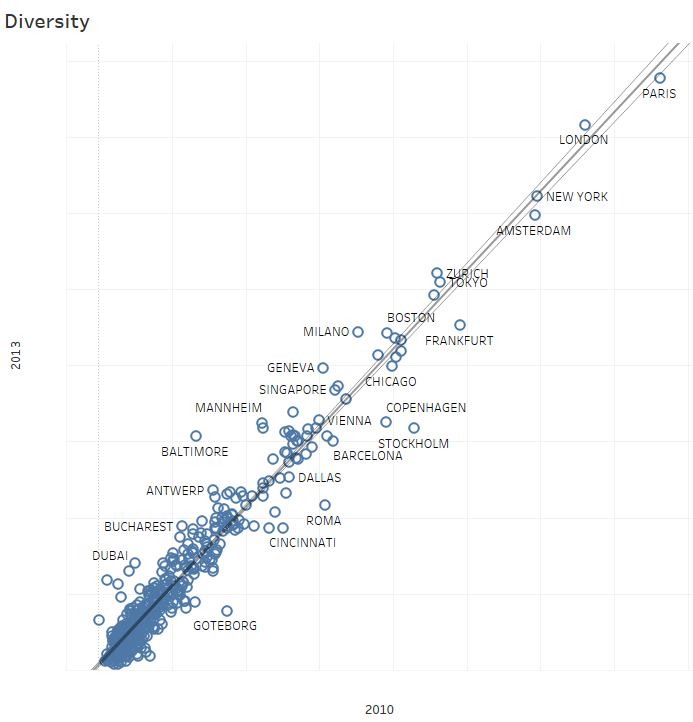
\includegraphics[width=0.8\linewidth]{city-network-diversity.png}
				\caption[Diversity plot of city networks]{Plotting \textit{Diversity} of cities in 2010 (x-axis) against 2013 (y-axis). The cities which are very close to the trend line have maintained their status. Cities below the trend line have decreased diversity from 2010 to 2013 whereas cities  above the trend line have increased diversity from 2010 to 2013.}
				\label{fig:city-network-diversity}
			\end{figure}
			
			\subsubsection{Strength}
			Figure \ref{fig:city-network-strength} shows the strength of cities in 2010 and 2013. Again, the cities which are close to the trend line have preserved their status over the years with some major cities like \textbf{Paris}, \textbf{New York} and \textbf{Amsterdam} showing this tendency. The cities which are below the trend line have decreased in terms of strength. Major cities affected are \textbf{Moscow}, \textbf{London}, \textbf{Frankfurt} and \textbf{Hong Kong} which are among the main financial centres in their own regions and it is interesting to see their decrease in strength. Cities which are above the trend line like \textbf{Philadelphia}, \textbf{Milan}, \textbf{Chicago} and \textbf{Tokyo} have increased their strength by increasing the weight of their connections to other cities. It is interesting to see a couple of cities from \textbf{China} (Beijing and Shanghai) in this list, as well as cities from \textbf{Brazil} (Sao Paulo) and \textbf{Romania} (Bucharest).
			
			\begin{figure}[H]
				\centering
				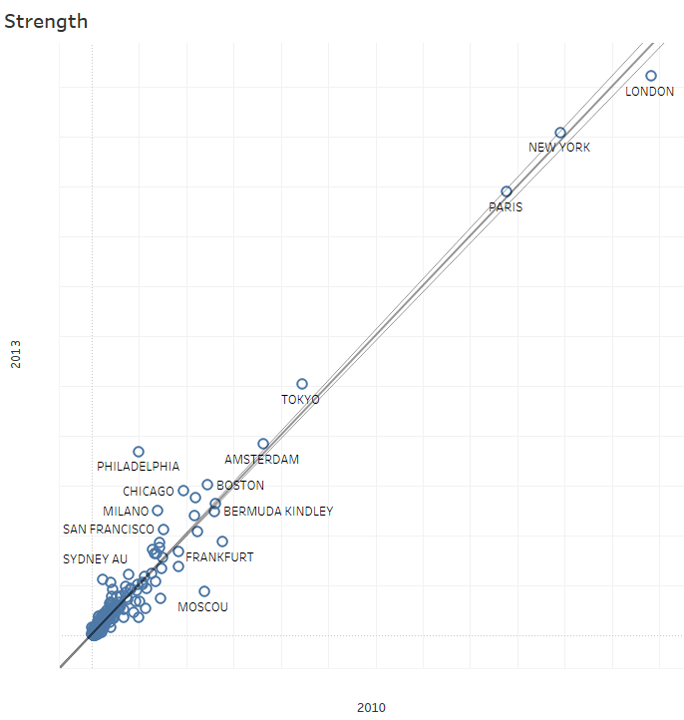
\includegraphics[width=0.8\linewidth]{city-network-strength}
				\caption[Strength plot of city networks]{Plotting \textit{Strength} of cities in 2010 (x-axis) against 2013 (y-axis). The cities which are very close to the trend line have maintained their status. Cities below the trend line have decreased strength from 2010 to 2013 whereas cities  above the trend line have increased strength from 2010 to 2013.}
				\label{fig:city-network-strength}
			\end{figure}
			
			\subsubsection{Centrality}
			Figure \ref{fig:city-network-centrality} shows the centrality of cities in 2010 and 2013. The enlarged image on the right shows only the top part for increased readability. The cities which are close to the trend line have similar centrality values for the two years with notable cities like \textbf{Frankfurt}, \textbf{Brussels}, \textbf{Vienna}, \textbf{Chicago} and \textbf{Saint Petersbourg}. Some of the cities which have decreased in terms of centrality are \textbf{Goteborg} (Sweden), \textbf{Graz} (Austria), \textbf{Salt Lake City} (USA) and \textbf{Kuwait}. Cities which have increased centrality include \textbf{Dubai} (UAE), \textbf{Salzburg} (Austria), \textbf{Baltimore} (USA) and \textbf{Penang} (Malaysia). It is interesting to note that there are a couple of cities each from \textbf{Russia}, \textbf{Korea}, \textbf{China} and \textbf{United Arab Emirates} in this list. \textbf{Eastern Europe} is also well represented by \textbf{Akrotiri} (Santorini in Cyprus), \textbf{Gdansk} (Poland), \textbf{Tirana} (Albania) and \textbf{Vilnius} (Lithuania) showing the emerging trend of these countries and regions.
			
			\begin{figure}[H]
				\centering
				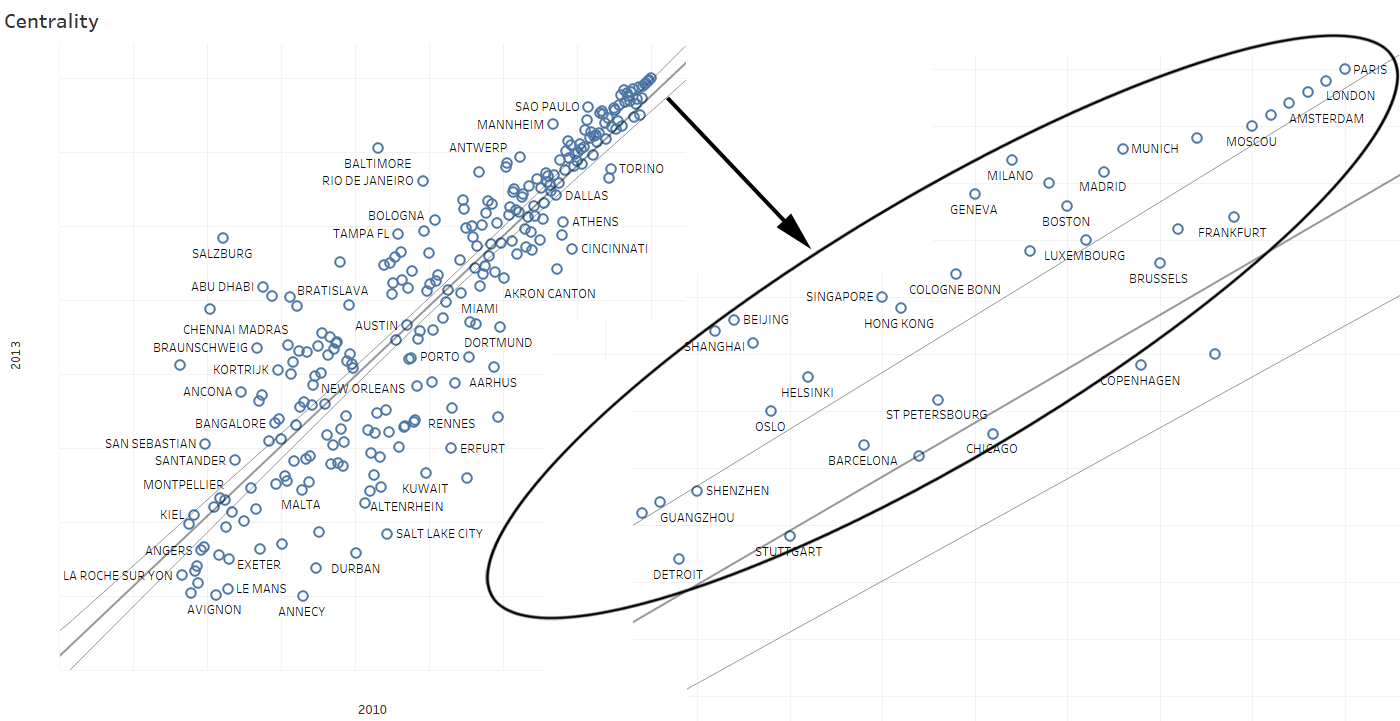
\includegraphics[width=0.8\linewidth]{city-network-centrality}
				\caption[Centrality plot of city networks]{Plotting \textit{Centrality} of cities in 2010 (x-axis) against 2013 (y-axis). The image on the right enlarges the top cities. Again the cities which are very close to the trend line have maintained their status. Cities below the trend line have decreased centrality from 2010 to 2013 whereas cities above the trend line have increased centrality from 2010 to 2013.}
				\label{fig:city-network-centrality}
			\end{figure}
			
			Figure \ref{fig:city-network-cumulative-centrality} shows the cumulative rank of cities in 2010 and 2013. The enlarged image on the right shows the top cities based on the cumulative ranking of the cities. The world’s top cities can easily be identified with most of the top performers in 2010 retaining their position in 2013. Cities like \textbf{Paris}, \textbf{London}, \textbf{New York} and \textbf{Tokyo} have fairly stable positions in both years. It means that despite some smooth changes in each of the dimensions, largest cities main- tain a very stable position. \textbf{Milan}, \textbf{Geneva}, \textbf{San Francisco} and \textbf{Baltimore} have improved their standings where cities like \textbf{Stockholm}, \textbf{Frankfurt}, \textbf{Copenhagen} and \textbf{Barcelona} have dropped their position.
			
			\begin{figure}[H]
				\centering
				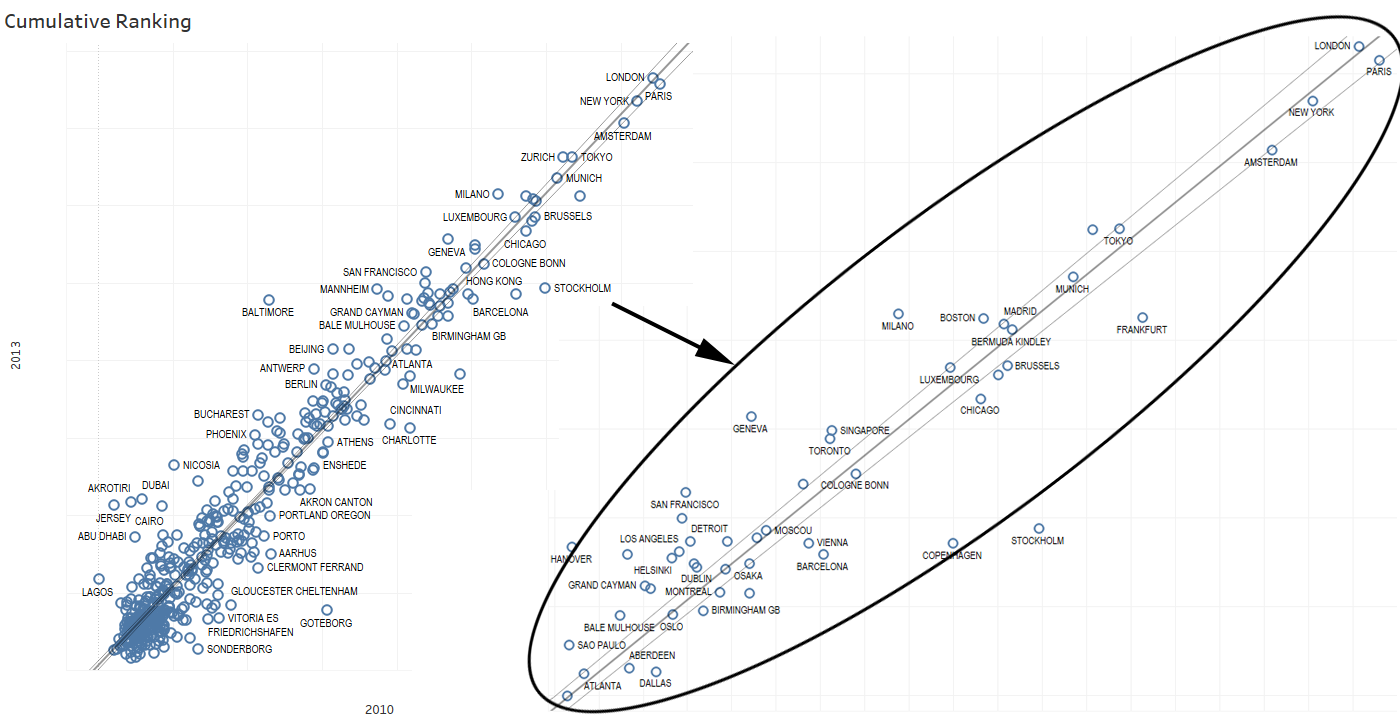
\includegraphics[width=0.8\linewidth]{city-network-cumulative-centrality}
				\caption[Cumulative ranking of cities for 2010 and 2013]{Plotting \textit{Cumulative Rank} of cities in 2010 (x-axis) against 2013 (y-axis). The image on the right shows the top cities zoomed-in. Again the cities which are very close to the trend line have maintained their status. Cities below the trend line have decreased the cumulative rank from 2010 to 2013 whereas cities above the trend line have increased cumulative rank from 2010 to 2013.}
				\label{fig:city-network-cumulative-centrality}
			\end{figure}
		
		Our findings are summarized in Figures \ref{fig:city-networks-top-cumulative-map}, \ref{fig:city-networks-top-positive-cumulative-map}, and \ref{fig:city-networks-top-negative-cumulative-map} in Appendix \ref{chp:figures} on a globe for better visualization.
		
		Cities which have been affected the most by the changes in global economic development of multinational firms from 2010 to 2013. Figure \ref{fig:city-networks-top-cumulative-map} shows the top 25 cities from the years 2010 and 2013. Three regions clearly stand out from the geographical perspective, North America, Western Europe and Eastern Asia. Moscow (Russia) and Sydney (Australia) are also among the top cities in the world. Cities from South America, all of Africa, South Asia and the Gulf are interestingly not part of this list.
		
		Figure \ref{fig:city-networks-top-positive-cumulative-map} and \ref{fig:city-networks-top-negative-cumulative-map} show the cities with the most positive and negative impact over the studied period.
		
		Comparing these cities with the top cities reveal how the world economy is changing in the context of multinational firms. Detailed results of all three metrics are given in section \ref{sec:appendix-B-city-networks} of Appendix \ref{chp:tables}. We discussed insights and details of a few cities from both the sets of cities with the highest positive and negative change in supplementary comments (Appendix \ref{sec:appendix-B-city-networks}). There are several factors that result in this change such as global economics, urban development, regional policies, international politics and social capital. Besides the general crisis affecting the whole cities’ network by a concentration in most of the former dominant regions, and the rise of new cities in emerging countries, the main factor explaining why some cities faced the crisis better than others can be found in their specialization in some growing economic sectors.
		
	The key observation from the above experiment from influence mining perspective is that albeit an abundance of methods and techniques and state-of-art being furthered each year, one method cannot qualify to be a gold standard in all real-world cases. Moreover, we observed that a primitive topological method such as Betweenness can also outperform state-of-art measures in certain cases.
	
	This finding leads us to take a collective approach instead of looking for one particular heuristic. The key question we aim to answer is if we can learn from multiple seed selection methods and train a single influential node identifier. The experiment discussed in next section is an attempt to use supervised machine learning, a data mining technique to achieve this objective.
	
%	\newpage
	
	%%%%%%%%%%%%%%%%%%%%%%
	%%% Experiment - 3 %%%
	%%%%%%%%%%%%%%%%%%%%%%
	\section{Influence maximization in complex networks through supervised machine learning}
	\label{sec:inf-max-machine-learning}
	Previous experiments evidently establish that a conventional way of inventing an algorithm to solve the influence mining problem work only for a particular set of use cases. Such techniques have to be evaluated before applying on a real-world use case. We propose that the answer lies in using data mining technique called supervised machine learning.
	
	The applications of machine learning emerging in every field is no surprise. However, the influence maximization domain surprisingly faces some scarcity. Among the few studies that exist, the prominent publications are quite specific, and often specific to social networks.
	
	Goyal et. al. \cite{goyal2010} focus on predicting the probability with which a user will propagate influence to individual neighbours in a network. Their proposed solution scans the log of user actions only twice and are able to learn three types of probabilistic models: static, continuous time and discrete time. Secondary contribution in this study is predicting the influence time. Finally, the results prove that continuous probabilistic model works better than static model. A common disadvantage with this solution is that it requires not only the network information, but also the log of actions performed by the nodes in the network. In addition to this, scanning the action logs twice can also be expensive in some situations as these logs tend to be huge in size.
	
	Guille et. al. \cite{guille2013} demonstrate how predictive analytics can be used to predict diffusion cascades in a social network. Their proposed model, T-BaSIC does not assume a fixed diffusion probability, but rather a time-dependent function. This temporal diffusion model is used create time series to describe how a topic originated and spread in a Twitter network in a closed set of users. The authors trained multiple classifiers to learn parameters for diffusion function, and opted Bayesian logistic regression classifier to define the diffusion function. The results show that int the information diffusion process, initially the volume of tweets is high against a topic, and then lowers with time following a wave pattern. Conclusively, the T-BaSIC method reduces the overall diffusion prediction error by 32.75\% in comparison with 1-time lag model proposed by Yang \cite{yang2011}.
	
	Zanin \cite{zanin2016} discusses the significance of applying data mining techniques in complex networks. The authors describe how data mining techniques can make use of structural patterns of individual nodes as well as whole network. Excerpts from this article are widely reflected in experiments we propose in the supervised machine learning experiment.
	
	Albeit these attempts, to the best of our knowledge there is lack of any published work which solves the influence mining problem using supervised machine learning on a complex networks of varying structural properties. These properties are thoroughly discussed in next sub-section.
	
		\subsection{Experiment settings}
		The primary focus is to provide a novel approach to identify influential nodes in complex networks. We attempt to develop a method which is widely applicable to networks with varying structural and nodal properties. The aim of this experiment is neither to invent a new machine learning algorithms, nor make performance comparisons between the existing machine learning algorithms.
		
			\subsubsection{Training data sets}
			The experiments discussed primarily consist of openly available real graphs as well as synthetically generated graphs. Moreover, unlike majority of studies, which use network data, user attributes, action logs and other information, we only use network’s structural properties that can be calculated by $G=(V,E)$, where $V$ is a set of vertices or nodes in the graph $G$, while $E$ is the set of edges or links connecting these vertices.
			
			Since it is vital to have variety in our data, we used networks from various domains, different sizes and different structural properties. The networks used in this study come from three sources:
			
			\begin{enumerate}
				\item Synthetic networks: We drew 6 random samples for each of the following types of complex networks using Igraph library \cite{igraph2006,barabasi1999,holme2002b} ranging from sizes: 10, 15, 20, 25, 30, 35, 40, 45, 100, 200, 300, 400, 500, 600, 700, 800, 900, 1000, 1500, and 2000. Thus creating 120 complex networks (scale free and small-world).
				
				\item Public networks: We used five of the frequently cited networks from various domains like biology and social networks, which are available online. Namely Zachary karate club \cite{zachary1977}, World trade \cite{smith1992}, Nematode \cite{white1986}, Political blog \cite{adamic2005} and Yeast protein \cite{jeong2001}.
				
				\item Extracted networks: we extracted two networks described as follows:
				
				\begin{itemize}
					\item Influence citations: network of paper citations on topic of influence mining till 2016. The data set was constructed by collecting a corpus of research articles on various topics of Influence mining. Each node in this network represents a unique article, while the edges represent citations between these articles.
					
					\item Twitter: network of users linked on Twitter, collected using snowball sampling. Starting with a reference user account (ID: seekme 94) in the Twitter network, a subset of Twitter’s network was extracted, in which each node is either a direct connection of reference account, or a connection at a distance of 1 degree. The edges represent interconnections between these nodes. The reference node was finally removed from the network.
				\end{itemize}
			\end{enumerate}
			
			This gives us a total of 367 networks for training and validation. Table \ref{tab:inf-max-machine-learning-training-graphs} shows basic statistics for all the real networks used for training the model. APL is Average Path Length, $\alpha$ is Power-law coefficient, CC is clustering coefficient and Avg. Deg is Average Degree. The variation in size of the networks, average path length, power law coefficient, clustering coefficient and average degree demonstrates how we have captured different network level structural properties for our training data set.
		
			\begin{table}[h]
				\centering
				\begin{tabular}{|l|l|l|l|l|l|l|}
					\hline
					\textbf{Network} & \textbf{Nodes} & \textbf{Edges} & \textbf{APL} & \textbf{$\alpha$} & \textbf{CC} & \textbf{Avg. Deg} \\ \hline
					Karate club        & 34   & 78    & 2.4 & 2.12 & 0.256 & 4.6  \\ \hline
					World trade        & 80   & 1000  & 1.7 & 2.56 & 0.460 & 25   \\ \hline
					Nematode           & 297  & 2359  & 2.5 & 3.29 & 0.181 & 15.9 \\ \hline
					Political blog     & 1222 & 19089 & 2.7 & 3.89 & 0.226 & 31.2  \\ \hline
					Yeast protein      & 1458 & 3941  & 6.8 & 3.24 & 0.052 & 5.4 \\ \hline
					Influence citation & 1254 & 1993  & 3.8 & 2.35 & 0.057 & 3.2  \\ \hline
					Twitter            & 894  & 2060  & 4.9 & 4.60 & 0.017 & 4.6  \\ \hline
				\end{tabular}%
				\caption{Real Networks used for training machine learning models}
				\label{tab:inf-max-machine-learning-training-graphs}
			\end{table}
			
			\subsubsection{Test data sets}
			In order to test the final model, following networks from various domains were used. Again, variation in their nodal as well as structural properties can be observed in Table \ref{tab:inf-max-machine-learning-test-graphs}. All these networks are also frequently used in different experiments and cited in the literature.
			
			\begin{table}[h]
				\centering
				\begin{tabular}{|l|l|l|l|l|l|l|}
					\hline
					\textbf{Network} & \textbf{Nodes} & \textbf{Edges} & \textbf{APL} & \textbf{$\alpha$} & \textbf{CC} & \textbf{Avg. Deg} \\ \hline
					Author   & 379    & 914    & 6.0 & 3.36 & 0.431 & 4.8  \\ \hline
					ITA 2000 & 3304   & 67195  & 4.0 & 1.69 & 0.249 & 40.7 \\ \hline
					AS-CAIDA & 26475  & 53381  & 3.9 & 2.09 & 0.007 & 4.0  \\ \hline
					JDK      & 6434   & 150985 & 2.1 & 2.01 & 0.011 & 46.9 \\ \hline
					Wordnet  & 145145 & 656230 & 5.5 & 2.47 & 0.096 & 9.0  \\ \hline
				\end{tabular}
				\caption{Real Networks used for testing classification models}
				\label{tab:inf-max-machine-learning-test-graphs}
			\end{table}
			
			\begin{itemize}
				\item Author NetScience: a coauthorship network of scientists working on network theory and experiment \cite{newman2006b}.
				
				\item ITA 2000: a reduced version of Air Transport network representing connections between airports through direct flights \cite{rozenblat2008}.
				
				\item AS-CAIDA: network of autonomous systems of the Internet connected with each other from the CAIDA project, collected in 2007 \cite{ascaida}.
				
				\item JDK Dependencies: a network of class dependencies in Java Development Framework v1.6 \cite{jdk}.
				
				\item Wordnet: a lexical network of English words in which each node represents a word and edges are relationships like synonym and antonyms \cite{fellbaum2012}.
				
			\end{itemize}
			
			
			\subsubsection{Machine learning models}
			In a relatively latest review paper, Fernandez et al. \cite{fernandez2014} argued that the real world classification problems do not require too many machine learning models after comparing 179 classifiers on 121 data sets. Analyzing the results of the best and worst performing models from different families, we used the following models for our experiment:
			
			\begin{enumerate}
				\item Logistic regression: Generalized Linear Model by Dobson \cite{dobson2018}, abbreviated as \textbf{GLM}.
				
				\item Decision Trees and Rule-Based: Recursive partitioning by \cite{breiman1984}, abbreviated as \textbf{RPart} and \textbf{C5.0}, an extended version of original C4.5 model by \cite{quinlan1993}. 
				
				\item Support Vector Machines: \textbf{SVM} model using Gaussian kernel from popular LibSVM library \cite{chang2011}.
				
				\item Boosting: Random Forests by \cite{breiman2001}, abbreviated as \textbf{RForest} and eXtreme Gradient model by \cite{chen2016}, abbreviated as \textbf{XGBoost}.
			\end{enumerate}
			
			From the data sets, the target variable tells whether the node was identified as influential by optimal/Greedy algorithm or not. The models are evaluated using accuracy measure, a standard way to compare the performance of machine learning models (see Equation \ref{eq:inf-max-accuracy}).
			
			\begin{equation}
				\label{eq:inf-max-accuracy}
				Accuracy=\frac{TP+TN}{TP+FP+TN+FN}
			\end{equation}
			
			Where $TP$ (true positives): number of nodes which were correctly classified as influential. $TN$ (true negatives): number of nodes which wore correctly classified as non-influential. $FP$ (false positive): number of nodes which were incorrectly classified as influential. $FN$ (false negative): number of nodes which were incorrectly classified as non-influential.
			
			\subsubsection{Modest computing power}
			The experiments were all conducted on a workstation laptop, consisting of quad-core CPU running at 3.6GHz in combination with 16GB RAM and 512GB storage. The modest computing power demonstrates that the solution does not require high-speed computational stations.
			
		\subsection{Influential node identification}
		The first step to train supervised machine learning models is to identify influential nodes in training data.
		
			\subsubsection{Influence maximization}
			In order to guarantee that the nodes we label as influential, in fact are influential, we used an exhaustive search to find the optimal solution (NP-hard) for networks of size less than 50 nodes (see Algorithm \ref{alg:influence-maximization}), and Hill-climbing based Greedy solution for larger networks (see Algorithm \ref{alg:influence-greedy-solution}). Opting for greedy algorithm was the next best method possible after an exhaustive search because finding the optimal solution for larger graphs is practically impossible in realistic time.
			
			\subsubsection{Influence test}
			In order to quantify the influence of a node, multiple methods exist, including diffusion test under both LT and IC models, resilience test \cite{cohen2000} which quantifies the network breakdown after a set of nodes is removed. Since the resilience test does not require any data other than network information, therefore this study uses resilience test as other similar studies \cite{holme2002,morone2015}. 

			Conventionally, the resilience test is a network decomposition function. In discrete time steps, one node (or a set of similar nodes) is removed from the network and we compute the largest connected component remaining in the network. This iteration is repeated until network completely decomposes. The quicker a method decomposes the network, the better its performance. In the underlying experiment, instead of single node a batch of $k$ nodes is removed in exactly one iteration and the size of the biggest connected component is measured.
			
			\subsubsection{Budget}
			Budget, or the number of influential nodes to identify, was fixed to 10\% for networks with nodes less than 50 and, 2.5\% for all other networks.
			
		\subsection{Training features}
		For a machine learning model to perform optimally, feature selection and data transformation are the key steps. For this experiment, we carefully chose a number of nodal and network level traits as training feature set:
		
		\begin{enumerate}
			\item Network traits: out of the numerous network traits which explain the structure of a network. Each trait has merits and demerits. This study chose the following 11 most commonly used network level traits as input to the training model, i.e. Network size, Edges, Highest Degree, Average Degree, APL, Clustering Coefficient, Diameter, Density, Average Distance, Number of Triads and Assortativity.
			
			\item Node centrality traits (see \ref{sec:related-seed-selection}): these traits define how central to the network certain node is. We included these five node centrality traits: Degree, Betweenness, Closeness, Eigenvector centrality and Eccentricity.
			
			\item Other heuristics (see \ref{sec:related-seed-selection}): in this category we picked three heuristics; we included Coreness due to its performance in identification of influential nodes as claimed by \cite{kitsak2010}, \cite{bae2014}. Batagelj proposed an algorithm with complexity $O(n)$ to compute coreness \cite{batagelj2003}. Secondly, we add Pagerank, the popular ranking algorithm developed by Google Inc. \cite{pagerank1999}. Third and last one is Collective Influence, because of two particular reasons: it identifies weak nodes, which act as bridges between strong influences; it is scalable to large networks. All of these heuristics exploit the topological information in order to grant ranking to a particular node.
		\end{enumerate}
		
		It is important to note that since not all attributes have bounded values between standard ranges; we normalized the unbounded attributes to standardize all data.
		
		\subsection{Results}
		First, we look at how each model performs on different sizes of networks. An ideal model should perform consistently well irrespective of size of the network. We then average the accuracy of each model on all the graphs in validation set.
		
		Figure \ref{fig:machine-learning-model-accuracy-by-size} illustrates the accuracy of classification models over different sizes of validation networks, horizontal axis represents size and vertical axis accuracy of models. Average accuracy is given in Figure \ref{fig:machine-learning-model-accuracy}.
		
		\begin{figure}[H]
			\centering
			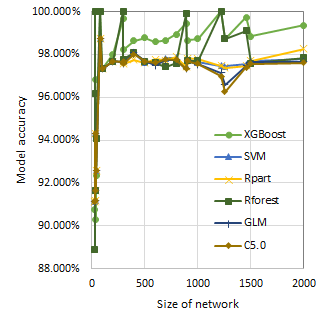
\includegraphics[width=0.7\textwidth]{machine-learning-model-accuracy-by-size}
			\caption[Accuracy of classification models]{Accuracy of classification models on various sizes of networks in validation set. Size of the networks are on horizontal axis, while the accuracy of each model on these sizes are on vertical axis.}
			\label{fig:machine-learning-model-accuracy-by-size}
		\end{figure}
		
		From Figure \ref{fig:machine-learning-model-accuracy}, it is evident that XGBoost has the highest accuracy overall on varying sizes of networks. We also observe that the performance of all models in small graphs is variable. However, XGBoost still outperformed other models on small networks. Therefore, we selected XGBoost based on its performance in comparison with other supervised machine learning models to evaluate networks in test data set.
		
		\begin{figure}[H]
			\centering
			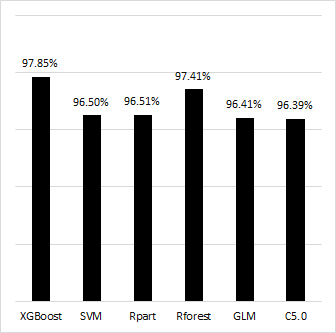
\includegraphics[width=0.5\textwidth]{machine-learning-model-accuracy}
			\caption[Average model accuracy on validation set]{Average accuracy of classification models on all networks in validation set}
			\label{fig:machine-learning-model-accuracy}
		\end{figure}
		
		The key objective of this study is to find out if a machine learning algorithm can outperform other heuristic methods in discovering influential nodes in networks of various sizes and structural properties. In order to test our hypothesis, we pass all the test networks to the XGBoost model to identify $k$ most influential nodes. The output obtained from the model is a probability against each node, which quantifies how strongly the model classified that particular node as influential. We pick the set of 5\% $k$ nodes of the highest probabilities and perform resilience test on the test networks. Resilience test is destructive; it is used to measure how much a network decomposed when a set of nodes is removed. After removing $k$ influential nodes identified by the model, we calculate the size of the largest connected component in the remaining network. Therefore the method, which identifies $k$ nodes that results in higher decomposition of the network qualifies as a better performer.
		
		The results shown in Figure \ref{fig:machine-learning-model-resilience} illustrate that the XGBoost model performed very well when compared with commonly used heuristics. In this figure, "size" on x-axis represents the number of nodes in the original test network, while other bars represent how large the network remained after removing 5\% $k$ influential nodes. Best results are highlighted with bold-italic text in the figure.
		
		\begin{figure}[H]
			\centering
			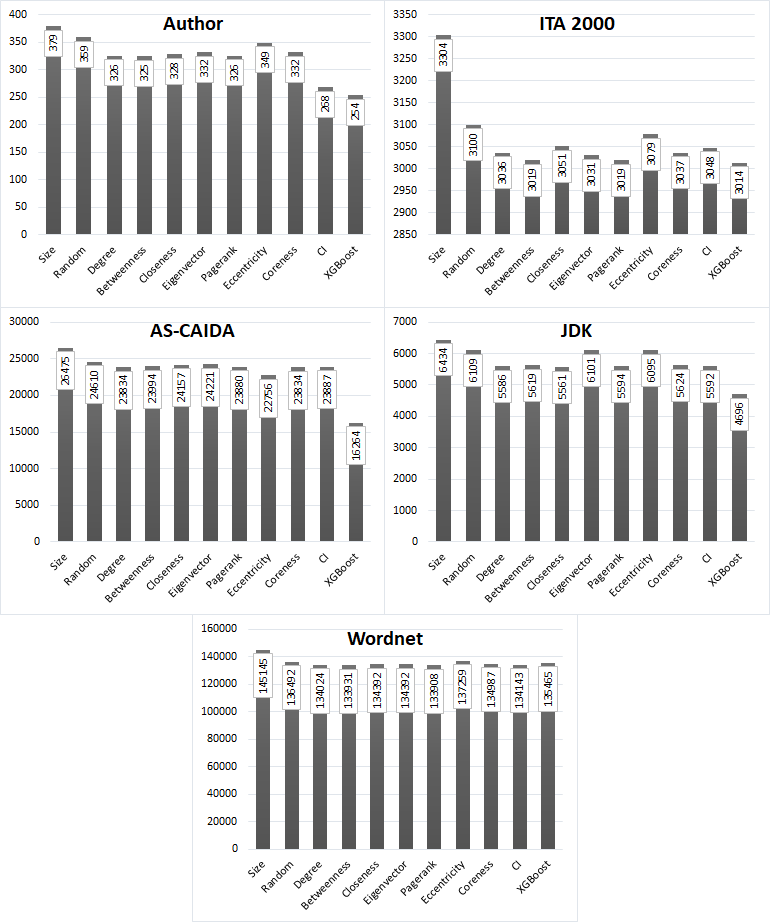
\includegraphics[width=0.7\textwidth]{machine-learning-model-resilience}
			\caption[Classification model vs other influence methods]{Comparison of influence mining methods against classification model. On x-axis are the methods under comparison. On y-axis is the number of nodes in largest component after removing $k$ nodes from the network}
			\label{fig:machine-learning-model-resilience}
		\end{figure}
		
			\subsubsection{Author}
			This is the smallest of all test networks. XGBoost model collapsed the largest connected component in the network to 254 nodes (removing 19 nodes).
			
			\subsubsection{ITA 2000}
			XGBoost showed best results with the size of largest connected component to 3014 nodes, but only marginally better than Pagerank and Betweenness centrality which reduced the size of the largest connected component to 3019 nodes (removing 165 nodes).
			
			\subsubsection{AS-CAIDA}
			A relatively large network, where XGBoost (16264 nodes) dominated other methods with significant margin. Eccentricity (22756 nodes) is the next best with a considerable difference (removing 1324 nodes).
			
			\subsubsection{JDK}
			Similar results with XGBoost (4696 nodes) can be observed (removing 322 nodes). It is interesting to note that in this particular network, Eigenvector centrality and Eccentricity are only slightly better than random method. Thus indicating that centrality based methods may not perform better universally.
			
			\subsubsection{Wordnet}
			Results on this -- largest -- network differs from others for XGBoost. The method that produced best results turned out to be Pagerank, which dismantled the network down to 133908 nodes on removing 7257 nodes. Followed closely by Betweenness (133931 nodes). The XGBoost model disappointingly fell below all other methods except Eccentricity and Random.
			
		Analyzing the results, although the XGBoost model stands on top, analysis on next best also reveals that there is no clear runner up method. For example, CI shows impressive results on Author network, but does not hold this performance on other networks. Table \ref{tab:inf-max-machine-learning-ranking} lists the influence methods and ranks using average ranking method. As observable, CI has 2nd rank in Author network, but fails on other networks; Betweenness and Pagerank perform equally well on ITA 2000, but do not hold this position for other networks; likewise, Eccentricity is impressive on AS-CAIDA network, but performs almost similar to random method on other networks.
		
		This observation also validates that the use of heuristic methods to identify influential nodes is highly dependent of various nodal and structural attributes and thus perform differently on different networks. Therefore, no heuristic can be considered as a generic algorithm to accurately identify influential nodes in a variety of complex networks.
		
		Another observation is that not all networks decompose with the same rate. For example, ITA 2000 network proved highly resilient by sustaining a size of 3014 (91\%) after removing influential nodes. On the other hand, AS-CAIDA reduced to 16264 (61\%). It is also evident that random methods perform poorly, as indicated by various other studies.
		
		Finally, coming to the case where machine learning model failed on Wordnet. A clear reason for such poor results is that in the training data, we had not provided the model with any network of such size. Here we find a learning limitation of the model, i.e. without providing ample data set which consists of all sizes of networks, the machine learning model fails to identify target nodes. Not only that, but as we observe in the results, it may perform about same as random selection.
		
		\begin{table}[h]
			\centering
			\begin{tabular}{|l|l|l|l|l|l|}
				\hline
				\textbf{Network} & \textbf{Author} & \textbf{ITA 2000} & \textbf{AS-CAIDA} & \textbf{JDK} & \textbf{Wordnet} \\ \hline
				\textbf{Random}       & 10  & 10  & 10  & 10 & 9   \\ \hline
				\textbf{Degree}       & 4.5 & 5   & 3.5 & 3  & 3   \\ \hline
				\textbf{Betweenness}  & 3   & 2.5 & 7   & 6  & 2   \\ \hline
				\textbf{Closeness}    & 6   & 8   & 8   & 2  & 5.5 \\ \hline
				\textbf{Eigenvector}  & 7.5 & 4   & 9   & 9  & 5.5 \\ \hline
				\textbf{Pagerank}     & 4.5 & 2.5 & 5   & 5  & 1   \\ \hline
				\textbf{Eccentricity} & 9   & 9   & 2   & 8  & 10  \\ \hline
				\textbf{Coreness}     & 7.5 & 6   & 3.5 & 7  & 7   \\ \hline
				\textbf{CI}           & 2   & 7   & 6   & 4  & 4   \\ \hline
				\textbf{XGBoost}      & 1   & 1   & 1   & 1  & 8   \\ \hline
			\end{tabular}
			\caption{Ranking comparison between the influence methods and classification model}
			\label{tab:inf-max-machine-learning-ranking}
		\end{table}
		
		The experiments and results not only validate the proposal by outperforming various conventional and state-of-art methods, but take us a step ahead in terms of prerequisites. The model which was trained for this study was based on synthetic networks, combined with some openly available network data sets. The classification model outperformed the competing methods in tested real world networks except in one instance. While machine learning can certainly help in various applications, it is important to note that training the model is computationally much more expensive than any other heuristic in comparison. It is assumed that anyone applying this solution aims to reuse the model on various networks, and multiple times. For simple one-time applications, the solution is still valid in terms of performance, but has a high computation overhead. Therefore, one of the key areas of optimization is selecting the right set of features which reduces the overall complexity while maintaining the high performance achieved.
		
		Following are the key finding from the above experiment:
		\begin{itemize}
			\item Machine learning is a plausible solution to identify influential nodes. Moreover, it can learn from synthetic networks and thus does not inherently require obtaining training set from variety of sources.
			
			\item The computation cost of learning a model is high, given that structural and nodal attributes have to be calculated for each network, as well as label the influential nodes via a highly efficient algorithm like Greedy.
			
			\item The method cannot be scaled without enhancing the training data first on large networks. Thus leading us to a case of deep learning on Big data.
			
			\item Finally, in order to pass target network to the model, all the meta features have to be also calculated for the target network. Even if all such features are calculated in linear time, the total time complexity will be $O(n*c)$, where $c$ is the number of features. Hence the technique cannot be scaled without comprehensive feature pruning.
		\end{itemize}	
		

	\section{Summary}
	\label{sec:inf-max-summary}
	The problem of Influence Maximization is NP-hard. However, because this function is both monotone and sub-modular, a Greedy solution can solve it with an approximation guarantee of 63\%. Most of the stat-of-art solutions are an extension or variants of this approach. Since Greedy solution scans the entire network from fresh perspective in each iteration, it is generic and can be used for all complex networks irrespective of their structural properties. Greedy solution suffers scalability problem due to its quadratic time complexity, thus leaving an open research question.
	
	%Real complex networks are all unique, but their properties can be mimicked within certain margin of error in synthetic networks. Such networks are a good way to study and benchmark the original networks which they replicate.
	
	Empirical analysis of various seed set selection methods confirms that there are structural dissimilarities between networks even from within the same domain. Social networks are all scale-free and small world, but still one influence method is effective on a particular social network, while fail on another one.
	
	There are various heuristics and techniques with claims to outperform other methods on a chosen set of networks, but even a well presented state-of-art method cannot guarantee consistency on all kinds of networks.
	
	In the absence of an ideal influence maximization method, machine learning is a suitable alternate solution to train a corpus of different networks on several seed selection methods and be used for a broader spectrum of networks than one particular method offers. Moreover, resilience test can also be used as a benchmark method to quantify the influence of a node or a set of nodes in a network alike influence test. Lack of use of resilience in literature spots a major research gap. \\
	
The experiments discussed in this chapter have revealed that due to dissimilarities in structure of different complex networks, it is not trivial to devise a general purpose algorithm which can perform uniformly better on all of them. Secondly, existing methods have been fixed in the way the influence process converges, i.e. budget given to identify number of nodes. Finally, a major research gap exists where researchers either use influence test, or resilience test to benchmark a method. We believe there is need for a framework which addresses these deficiencies.
